\documentclass{beamer}
\usepackage{animate}
\usepackage{graphics}
\usepackage{amsmath}
\usepackage{listings}  % Include the listings package for code
\usetheme[sectionpage=none, progressbar=frametitle, numbering=fraction]{metropolis}  % Use metropolis theme  
\usetheme[sectionpage=none, progressbar=frametitle, numbering=fraction]{metropolis}  % Use metropolis theme  
\title{Mathematik in der Spielentwicklung}
\date{}
\author{}  % Remove if not needed
\institute{}  % Remove if not needed



\usepackage[utf8]{inputenc}  % Add this for UTF-8 encoding support

\setbeamertemplate{title separator}{\vskip0.2cm\hrule height 0.5pt width \linewidth\hspace{0.2cm}\vskip0.3cm}  
\setbeamercolor{title separator}{fg=orange}  % Set color for title separator

\titlegraphic{\includegraphics[width=0.3\textwidth]{HsH.png}} 

\begin{document}
	
	\maketitle
	
\begin{frame}
	\frametitle{Gliederung}
	\centering
	\begin{minipage}{0.5\textwidth}
		\centering
		\rotatebox{90}{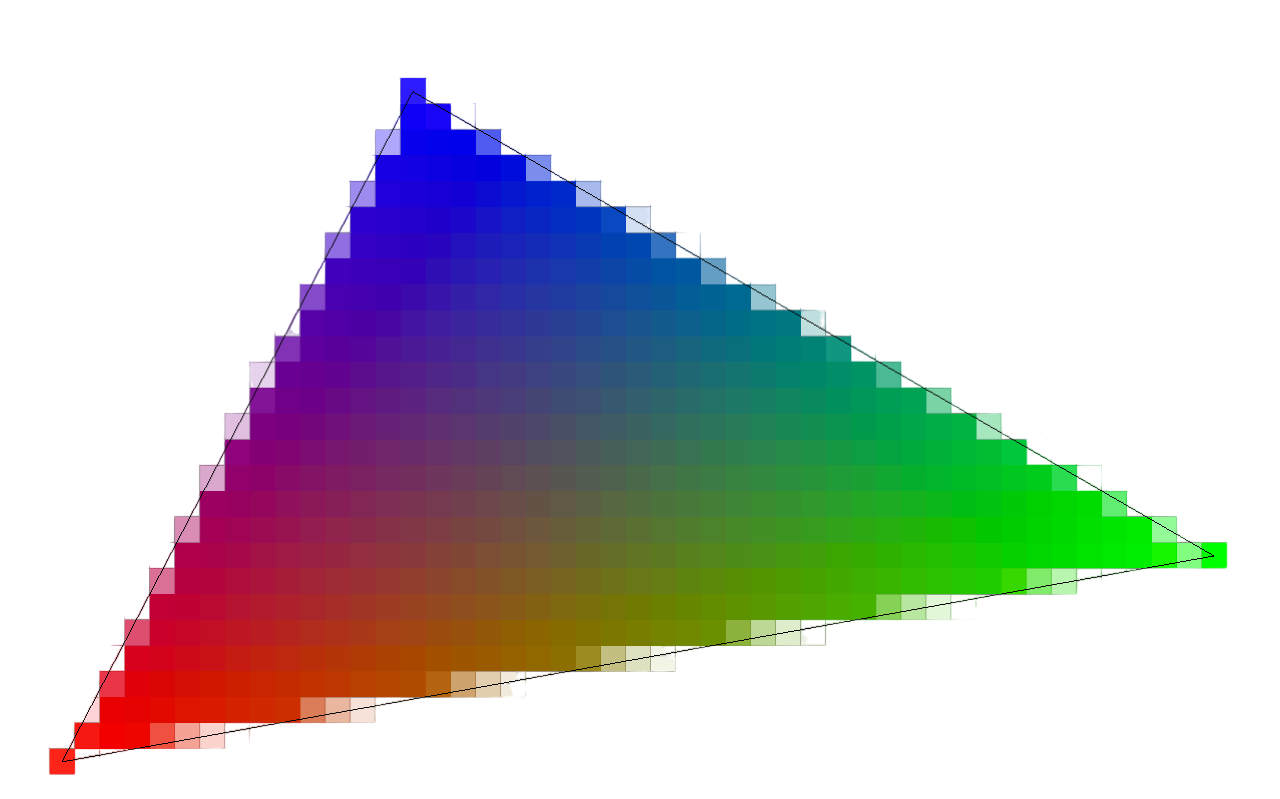
\includegraphics[width=7cm]{ii-.png}}
	\end{minipage}%
	\begin{minipage}{0.45\textwidth}
		\begin{itemize}
			\item Rasterung
			\item Rotatiomatrix
			\item Kreuzprodukt
		\end{itemize}
	\end{minipage}
\end{frame}

\begin{frame}
	\frametitle{Rasterung}
		\textmd{\small Das Bild auf der rechten Seite sieht ziemlich blockig aus, aber im wirklichen Leben sind die Pixel in der Regel viel kleiner als hier, so dass das Bild glatt aussieht. Je kleiner die Pixel sind, desto glatter ist das Bild. Unser Ziel ist es, vom Dreieck auf der linken Seite zu den Pixeln auf der rechten Seite zu gelangen, damit wir es auf den Bildschirm bringen können.} \\
		\vspace{0.3cm} % Adjust spacing between text and image
		\centering
		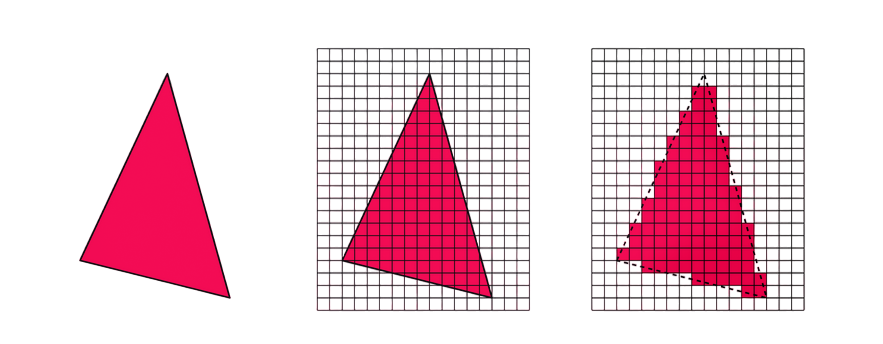
\includegraphics[width=10cm]{raster-.png}

\end{frame}

\begin{frame}
	\frametitle{\phantom{}}
	\vspace{-1cm}
	\textmd{\small Warum Dreiecke? Dafür gibt es mehrere Gründe, aber der Hauptgrund ist, dass es die einfachste Form ist, aus der man jede beliebige Form machen kann. Wenn man genug Dreiecke hat, kann man jede beliebige Form herstellen.} \\
	\vspace{0.3cm} % Adjust spacing between text and image
	\centering
	
\includegraphics[width=10cm]{triangles-.png}

\end{frame}

\begin{frame}
	\frametitle{Flächeninhalt eines Dreiecks}
	\vspace{-2.8cm}
	\begin{block}{Standartformel}
		\vspace{4mm}
		\textmd{\small Wenn wir an die Flächeninhalt eines Dreiecks denken, verwenden wir in der Regel die Formel:}
		\[
		\text{A} = \frac{\text{Grundseite} \times \text{Höhe}}{2}
		\]
	\end{block}
\end{frame}
\begin{frame}
	\frametitle{\phantom{}}
	\begin{block}{Standardformel}
		\vspace{4mm}
		\textmd{\small Wenn wir an die Fläche eines Dreiecks denken, verwenden wir in der Regel die Formel:}
		\[
		\text{Area} = \frac{\text{Grundseite} \times \text{Höhe}}{2}
		\]
	\end{block}
	\vspace{-5mm}
	\begin{block}{Gaußsche Trapezformel}
		\vspace{4mm}
		\textmd{\small Wenn jedoch die Koordinaten der Eckpunkte des Dreiecks bekannt sind, kann man den Flächeninhalt mit Hilfe der Gaußsche Trapezformel berechnen.}
		\[
		\text{A} = |\frac{(x_{b} - x_{a})(y_{c} - y_{a}) - (y_{b} - y_{a})(x_{c} - x_{a})}{2}|
		\]	
		\end{block}
\end{frame}
\begin{frame}
	\frametitle{\phantom{}}	
	\begin{figure}
		\centering
		
\includegraphics[width=8cm]{chicken.png}
	\end{figure}
\end{frame}

\begin{frame}
	\frametitle{\phantom{}}	
	\begin{figure}
		\centering
		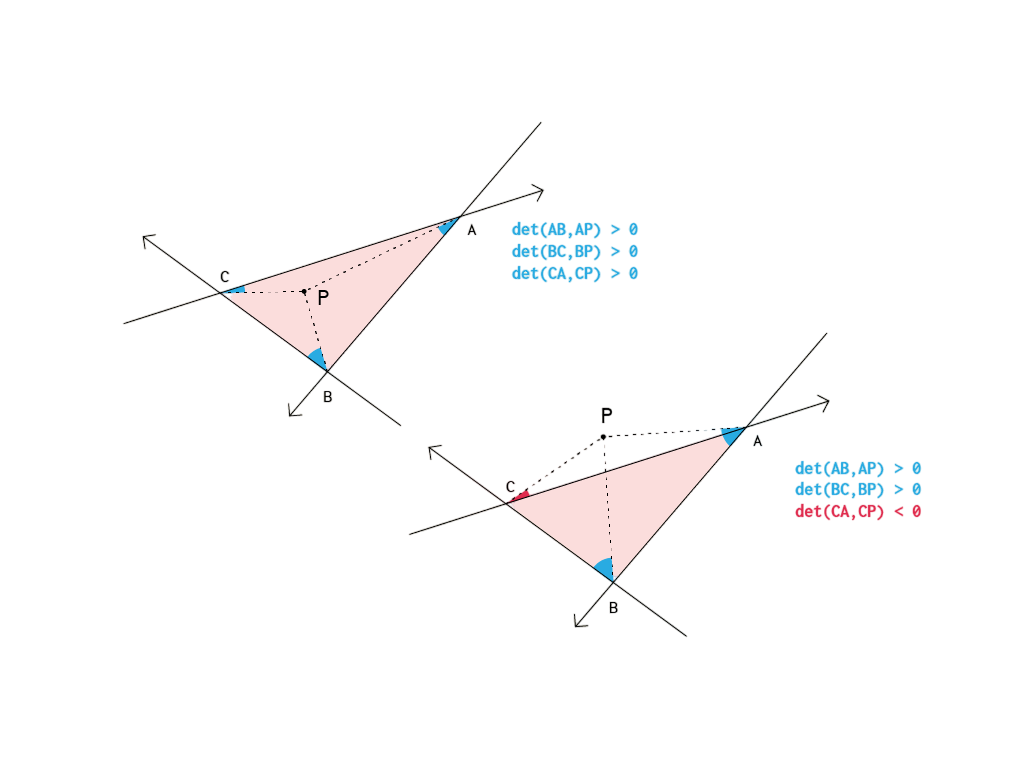
\includegraphics[width=10cm]{points-.png} 
	\end{figure}
\end{frame}

\begin{frame}
	\frametitle{Rotationmatrix}
		\vspace{-2.8cm}
		\textmd{\small Es gibt viele Möglichkeiten, mit 3D-Punkten umzugehen, aber die einfachste ist die Multiplikation mit einer Matrix. Der Punkt wird als ein 3 x 1 Vektor dargestellt. Die Transformation ist dann einfach die Multiplikation des 3 x 1-Vektors mit einer 3 x 3-Matrix.} \\
	\vspace{0.3cm}
	\centering
	$ AB = (a_{x}, a_{y}, a_{z})
	\begin{pmatrix}
		b_{xx} & b_{xy} & b_{xy} \\
		b_{yx} & b_{yy} & b_{yz} \\
		b_{zx} & b_{zy} & b_{zz} \\
	\end{pmatrix}
	$	
	\end{frame}
	
\begin{frame}
	\frametitle{Rotationmatrix}
	\vspace{0.3cm}
	\textmd{\small Es gibt viele Möglichkeiten, mit 3D-Punkten umzugehen, aber die einfachste ist die Multiplikation mit einer Matrix. Der Punkt wird als ein 3 x 1 Vektor dargestellt. Die Transformation ist dann einfach die Multiplikation des 3 x 1-Vektors mit einer 3 x 3-Matrix.} \\
	\vspace{0.5cm}
	\centering
	$ AB = (a_{x}, a_{y}, a_{z})
	\begin{pmatrix}
		b_{xx} & b_{xy} & b_{xy} \\
		b_{yx} & b_{yy} & b_{yz} \\
		b_{zx} & b_{zy} & b_{zz} \\
	\end{pmatrix}
	$
	\vspace{0.5cm}
	\[
	\quad
	\tiny _{xy}
	\begin{pmatrix}
		\cos(a) & -\sin(a) & 0 \\
		\sin(a) & \cos(a) & 0 \\
		0 & 0 & 1
	\end{pmatrix}
	\quad \! _{yz}
	\begin{pmatrix}
		1 & 0 & 0 \\
		0 & \cos(a) & \sin(a) \\
		-\sin(a) & \cos(a) & 1 
	\end{pmatrix}
	\quad \! _{xz}
	\begin{pmatrix}
		\cos(a) & 0 & -\sin(a) \\
		0 & 1 & 0 \\
		\sin(a) & 0 & \cos(a)
	\end{pmatrix}
	\]
	
\end{frame}
	
\end{document}